\section{Zadanie 1}
W celu sprawdzenia poprawno�ci warto�ci sygna��w w punkcie pracy pobudzili�my obiekt sygna�em o sta�ej warto�ci r�wnej $U_\mathrm{pp} = 0$, przy sta�ym zak��ceniu $Z_\mathrm{pp} = 0$. Spodziewana warto�� wyj�cia to $Y_\mathrm{pp} = 0$.

Zadanie wykonali�my przy u�yciu skryptu \verb+zad1.m+, kt�ry symuluje badan� sytuacj�. Przy opisanym wy�ej pobudzeniu obiekt, zgodnie z oczekiwaniami, stabilizuje si� w $Y_\mathrm{pp} = 0$ ($Rys. 2.1$).
\begin{figure}[h]
\centering
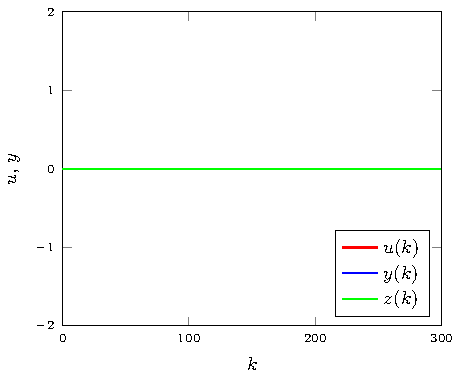
\includegraphics[scale=1]{rysunki/zad1_punktpracy}
\caption{Odpowied� procesu na pobudzenie sta�ym sygna�em i zak��ceniem r�wnym \num{0}.}
\end{figure}